\documentclass[12pt]{article}

% Modelo oficial da SBC para artigos (sbc-template.sty e sbc.bst, baixados de
% https://www.sbc.org.br/wp-content/uploads/2024/07/modelosparapublicaodeartigos.zip).
% O modelo já carrega geometry, times, caption e titlesec.
% (o babel precisa vir ANTES do sbc-template: com o hyperref carregado, a
% ordem inversa quebra a compilação no \begin{document})
\usepackage[T1]{fontenc}
\usepackage[utf8]{inputenc}
\usepackage[brazil]{babel}
\usepackage{sbc-template}

\usepackage{graphicx,url}
\usepackage{booktabs}
\usepackage{adjustbox}
\usepackage{amsmath,amssymb}
\usepackage{float}
\usepackage[hidelinks]{hyperref}

\graphicspath{{figuras/}}
\sloppy

\title{Análise Empírica e Otimização para o Caixeiro Viajante:\\
Branch-and-Bound, Twice-around-the-tree e Christofides}

\author{Juliano Gomes de Rezende\inst{1}}

\address{Departamento de Ciência da Computação\\
  Universidade Federal de Minas Gerais (UFMG) -- Belo Horizonte -- MG -- Brasil
  \email{julianorezende09@gmail.com}
}

\begin{document}

\maketitle

\begin{abstract}
We implement, audit, refactor and empirically profile an exact Branch-and-Bound
(B\&B) solver alongside the Twice-around-the-tree and Christofides approximation
algorithms for the Geometric Traveling Salesperson Problem across 15 TSPLIB
instances and 159 synthetic adversarial instances with known exact optima.
Subroutine-level profiling reveals that blossom matching grows as $N^{2.89}$ and
dominates Christofides, whereas vectorized $O(n^2)$ routines scale as $N^{1.2}$
due to Python interpreter overhead; disabling garbage collection did not alter
any fitted complexity exponent. Under blind child ordering, the convex-hull
insertion warm-start reduced expanded nodes by 41 times relative to the trivial
tour. The 1-tree lower bound collapses at $N=22$, while Held-Karp solves every
instance in the test suite. Finally, the fraction of points on the convex hull
is the strongest geometric predictor of the approximation gap.
\end{abstract}

\begin{resumo}
Implementamos, auditamos, refatoramos e instrumentamos em nível de subrotina um
Branch-and-Bound (B\&B) exato e os algoritmos aproximados Twice-around-the-tree
e Christofides para o Problema do Caixeiro Viajante Geométrico em 15 instâncias
da TSPLIB e 159 instâncias sintéticas adversariais com ótimo exato conhecido. O
emparelhamento blossom cresce como $N^{2{,}89}$ e domina o custo do Christofides,
enquanto rotinas $O(n^2)$ vetorizadas comportam-se como $N^{1{,}2}$ pelo custo
fixo do interpretador Python; desligar o coletor de lixo não alterou nenhum
expoente ajustado. Com ordenação cega de filhos, o warm-start do fecho convexo
expandiu 41 vezes menos nós que a solução trivial. O limite de 1-árvore colapsa
em $N=22$, enquanto Held-Karp resolve todas as instâncias. A fração de pontos
no fecho convexo é a característica geométrica que mais explica o gap.
\end{resumo}


\section{Introdução}

O Problema do Caixeiro Viajante (TSP) pede o ciclo hamiltoniano de menor
custo num grafo completo com pesos. Ele é NP-difícil: algoritmos exatos
levam tempo exponencial no pior caso, e na prática são usados
aproximativos com garantia de qualidade quando a métrica satisfaz a
desigualdade triangular~\cite{applegate2006}. São eles o
Twice-around-the-tree (TATT), com fator 2, e o
Christofides~\cite{christofides1976}, com fator 1,5. Este trabalho
implementa três algoritmos e os avalia empiricamente:
\begin{itemize}
  \item um Branch-and-Bound (B\&B) exato com três limites inferiores (duas
    menores arestas, 1-árvore e Held-Karp~\cite{heldkarp1970,heldkarp1971});
  \item o TATT;
  \item o Christofides.
\end{itemize}
O foco não é só a escrita do código, mas também a \emph{auditoria} e a
\emph{modelagem empírica} do desempenho.

As contribuições são quatro.
\begin{enumerate}
  \item \emph{Profiling por subrotina e complexidade empírica}
    (Seção~\ref{sec:complexidade}). Mostramos onde a complexidade teórica
    aparece (o blossom, $N^{2{,}89}$) e onde ela é mascarada pelo
    interpretador (Prim $O(n^2)$ medido como $N^{1{,}2}$). Também mostramos
    que o garbage collector não distorce as curvas, mas cópias de memória
    sim.
  \item \emph{Impacto do warm-start} nos nós expandidos e podados do B\&B
    (Seção~\ref{sec:warmstart}). O ganho depende da ordem de visita dos
    filhos: quando a busca é cega, o fecho convexo reduz a árvore em
    41$\times$; quando os filhos são ordenados pelo limite, o UB inicial
    quase não importa.
  \item \emph{Análise de sensibilidade} (Seção~\ref{sec:sens}). O gap de
    cada aproximativo foi relacionado a features geométricas e da MST em
    174 instâncias com ótimo exato, 159 delas sintéticas e geradas para
    serem adversariais.
  \item \emph{Auditoria} (Seção~\ref{sec:auditoria}). Comparamos o código
    refatorado com uma versão ingênua e registramos uma revisão cruzada
    entre dois modelos de IA, que encontrou erros
    de \emph{medição}, e não de algoritmo.
\end{enumerate}

\section{Implementação, profiling e auditoria}\label{sec:impl}

Tudo foi implementado em Python~3.11 com NumPy. O NetworkX~\cite{hagberg2008}
é usado apenas no emparelhamento perfeito de peso mínimo do Christofides, e o
scikit-learn~\cite{pedregosa2011} apenas na análise. O código está organizado
em \texttt{tsp/}: leitor da TSPLIB, MST, heurísticas, aproximativos, B\&B,
features e profiler. Os experimentos ficam em \texttt{run\_*.py},
\texttt{profile\_scaling.py} e \texttt{audit\_naive.py}, e a análise em
\texttt{analise/}. Há 103 testes automatizados, que comparam com força
bruta, com o SciPy e com os ótimos e tours publicados da TSPLIB.

\subsection{Instâncias e distâncias}
O enunciado pede instâncias EUC\_2D com $N\in[10,75]$, mas a TSPLIB só tem
três nessa faixa (eil51, berlin52 e st70). Vários exemplos do próprio
enunciado são de outros tipos: ulysses16 é GEO, gr24, fri26 e swiss42 são
EXPLICIT, e att48 é ATT. Usamos 15 instâncias de 14 a 70 vértices
(Tabela~\ref{tab:instancias}), cada uma com a distância oficial do seu
tipo~\cite{reinelt1991}. A validação é que o custo de cada \texttt{.opt.tour}
publicado coincide com o ótimo publicado.

A regra de 80\% das instâncias com $N\le 40$ também não pode ser cumprida
com a TSPLIB, que só tem nove instâncias simétricas com $N\le40$. Usamos
todas as nove (60\% do conjunto). As instâncias EXPLICIT não têm
coordenadas. Para elas, coordenadas 2D foram obtidas por escalonamento
multidimensional clássico (MDS) da matriz de distâncias, e são usadas
\emph{apenas} nas features geométricas e na heurística do fecho convexo.
Para compensar o conjunto pequeno na análise de sensibilidade, geramos
instâncias sintéticas adversariais (Seção~\ref{sec:sens}).

\begin{table}[htb]
\centering
\caption{Instâncias da TSPLIB usadas. Geometria: origem das coordenadas das features geométricas. Viol. triangular: fração das triplas $(i,j,k)$ com $d(i,k)>d(i,j)+d(j,k)$.}
\label{tab:instancias}
\small
\begin{adjustbox}{max width=\linewidth}
\begin{tabular}{lrlrlrrr}
\toprule
Instância & $N$ & Tipo & Ótimo & Geometria & Fração no fecho & Clark-Evans & Viol. triangular \\
\midrule
burma14 & 14 & GEO & 3323 & coordenadas & 0{,}36 & 1{,}13 & 0{,}00\% \\
ulysses16 & 16 & GEO & 6859 & coordenadas & 0{,}44 & 1{,}10 & 0{,}00\% \\
gr17 & 17 & EXPLICIT & 2085 & MDS & 0{,}35 & 0{,}99 & 3{,}28\% \\
gr21 & 21 & EXPLICIT & 2707 & MDS & 0{,}38 & 1{,}10 & 2{,}61\% \\
ulysses22 & 22 & GEO & 7013 & coordenadas & 0{,}32 & 0{,}95 & 0{,}00\% \\
gr24 & 24 & EXPLICIT & 1272 & MDS & 0{,}29 & 1{,}18 & 4{,}61\% \\
fri26 & 26 & EXPLICIT & 937 & MDS & 0{,}35 & 1{,}09 & 0{,}17\% \\
bayg29 & 29 & EXPLICIT & 1610 & DISPLAY\_DATA & 0{,}24 & 1{,}33 & 0{,}00\% \\
bays29 & 29 & EXPLICIT & 2020 & DISPLAY\_DATA & 0{,}24 & 1{,}33 & 2{,}24\% \\
dantzig42 & 42 & EXPLICIT & 699 & DISPLAY\_DATA & 0{,}19 & 1{,}07 & 3{,}66\% \\
swiss42 & 42 & EXPLICIT & 1273 & MDS & 0{,}21 & 1{,}06 & 0{,}16\% \\
att48 & 48 & ATT & 10628 & coordenadas & 0{,}23 & 1{,}01 & 0{,}00\% \\
eil51 & 51 & EUC\_2D & 426 & coordenadas & 0{,}16 & 1{,}52 & 0{,}21\% \\
berlin52 & 52 & EUC\_2D & 7542 & coordenadas & 0{,}15 & 0{,}98 & 0{,}12\% \\
st70 & 70 & EUC\_2D & 675 & coordenadas & 0{,}14 & 1{,}04 & 0{,}23\% \\
\bottomrule
\end{tabular}
\end{adjustbox}
\end{table}


\subsection{Estruturas de dados e algoritmos}

\paragraph{Matriz de distâncias.} A matriz é densa ($n\times n$,
\texttt{float64}) e representa exatamente as distâncias inteiras da TSPLIB
(até $2^{53}$). Ela é \texttt{float} porque o limite de Held-Karp soma
penalidades reais. Uma cópia com $+\infty$ na diagonal evita testes
$i\neq j$ nos laços.

\paragraph{MST (Prim $O(n^2)$).} O grafo é completo, então Prim com vetor de
chaves é ótimo para grafo denso: $O(n^2)$, sem materializar as $n(n-1)/2$
arestas, como faria o Kruskal, e sem o $\log n$ do heap. Cada uma das $n$
iterações é uma operação vetorizada sobre o vetor de chaves.

\paragraph{Twice-around-the-tree.} Pré-ordem iterativa da MST (pilha
explícita), que equivale a percorrer cada aresta da árvore duas vezes e pular
os repetidos. O custo é $\le 2\,\mathrm{MST}\le 2\,\mathrm{OPT}$ sob a
desigualdade triangular.

\paragraph{Christofides~\cite{christofides1976}.} O algoritmo calcula a MST,
toma os vértices de grau ímpar ($k$ deles) e encontra um emparelhamento
perfeito de peso mínimo entre eles. Depois monta um circuito euleriano pelo
algoritmo de Hierholzer, com ponteiro por vértice para a próxima aresta
(cada aresta é examinada $O(1)$ vezes), e por fim aplica os atalhos. O
NetworkX só oferece emparelhamento de peso \emph{máximo} (blossom de
Edmonds~\cite{edmonds1965,galil1986}, $O(k^3)$). Usamos então
$w'(u,v)=C-d(u,v)$ com $C>\max d$ e \texttt{maxcardinality=True}: como todo
emparelhamento perfeito tem $k/2$ arestas, maximizar $\sum w'$ equivale a
minimizar $\sum d$. Também implementamos um emparelhamento guloso, que
escolhe as arestas em ordem crescente de peso em $O(k^2\log k)$, mas perde a
garantia de 1,5. Ele serve para medir o custo e a qualidade do blossom.

\paragraph{Heurísticas de warm-start.} São três:
\begin{itemize}
  \item \emph{trivial}: o tour $1\to2\to\dots\to n\to 1$;
  \item \emph{vizinho mais próximo}: $O(n^2)$, com máscara vetorizada dos
    visitados;
  \item \emph{inserção a partir do fecho convexo}: o fecho é calculado pela
    cadeia monótona de Andrew~\cite{andrew1979}, em $O(n\log n)$. Os
    vértices internos entram por inserção mais barata~\cite{rosenkrantz1977}.
    O tour é uma lista ligada (\texttt{succ}), e cada vértice de fora guarda
    em cache sua melhor inserção. Inserir $k$ entre $a$ e $b$ destrói só a
    aresta $(a,b)$, então só quem tinha $(a,b)$ como melhor aresta é
    recalculado contra o tour inteiro; os demais comparam apenas com as duas
    arestas novas.
\end{itemize}
Os aproximativos (TATT e Christofides) completam as cinco estratégias.

\subsection{Branch-and-Bound}

\paragraph{Espaço de busca.} Um nó é um caminho parcial
$P=(0,v_1,\dots,v_k)$, com $R$ o conjunto dos vértices não visitados. Fixar o
vértice inicial elimina as $n$ rotações equivalentes de cada tour. Os filhos
são $P+(c)$ para $c\in R$, e o nó com $|R|=1$ fecha o tour. Como os custos
são inteiros, um nó só melhora a incumbente $\mathrm{UB}$ se
$\lceil \mathrm{LB}\rceil\le \mathrm{UB}-1$; podamos quando
$\lceil\mathrm{LB}-10^{-6}\rceil\ge\mathrm{UB}$, com tolerância para o erro
de ponto flutuante.

\paragraph{Limites inferiores.} Todos são calculados para os $|R|$ filhos de
uma vez. Seja $R'=R\setminus\{c\}$.
\begin{itemize}
  \item \emph{Duas menores arestas} (\texttt{twomin}, o limite clássico
    de~\cite{levitin2012}). Somam-se, para cada vértice, as arestas fixadas
    no caminho ou as duas mais baratas incidentes a ele, e o total é dividido
    por 2.
  \item \emph{1-árvore} (\texttt{onetree}). Ainda falta um caminho
    hamiltoniano $c\to r_1\to\dots\to r_j\to 0$ passando por todo $R'$.
    Tirando as duas arestas das pontas, sobra uma árvore geradora de $R'$:
    \[
      \mathrm{LB}(c)=d(P)+d(v_k,c)+\mathrm{MST}(R')
      +\min_{r\in R'} d(c,r)+\min_{r\in R'} d(r,0).
    \]
  \item \emph{Held-Karp} (\texttt{hk})~\cite{heldkarp1970,heldkarp1971}. É o
    mesmo limite sobre os custos penalizados $w_{ij}=d_{ij}+\pi_i+\pi_j$.
    Todo tour tem grau 2 em todo vértice, então
    $w(\text{tour})=d(\text{tour})+2\sum\pi$, e qualquer limite em $w$ vale
    para $d$ subtraindo $2\sum\pi$. As penalidades são otimizadas uma única
    vez, na raiz, por subgradiente da relaxação Lagrangiana da 1-árvore:
    $g_v=\mathrm{grau}_v-2$ e passo de Polyak
    $t=\lambda(\mathrm{UB}-L(\pi))/\lVert g\rVert^2$. O $\lambda$ começa em 2
    e cai pela metade após $\max(5,n/5)$ iterações sem melhora, com no máximo
    $50n$ iterações. O UB que calibra o passo é sempre o do vizinho mais
    próximo, para que o limite (e portanto a poda) não dependa do warm-start.
\end{itemize}
Os limites dos filhos exigem $\mathrm{MST}(R\setminus\{c\})$ para cada
$c\in R$. Em vez de $|R|$ execuções do Prim, com $|R|^2$ iterações do
interpretador, rodamos os $|R|$ Prims \emph{em lote}. Uma matriz de chaves
$|R|\times|R|$ é relaxada com uma operação NumPy por iteração, de modo que o
laço Python tem $|R|-2$ iterações. O custo aritmético continua
$O(|R|^3)$ por nó.

\paragraph{Estratégia de busca.} A estratégia padrão é a busca em
profundidade (DFS) recursiva, com um único vetor booleano de visitados e um
único caminho, ambos modificados no lugar. A memória é $O(n^2)$ (pilha de
recursão mais um vetor de limites por nível), contra a memória exponencial
do best-first. Os filhos podem ser visitados em ordem crescente de LB
(\emph{filhos por LB}), o que dá à DFS um comportamento parecido com o do
best-first, ou na ordem dos índices (\emph{filhos por índice}). No segundo
caso, a DFS depende só do UB para podar, o que isola o efeito do warm-start.
Com filhos ordenados, ao podar um filho podamos também todos os irmãos
seguintes. O best-first também está implementado: um heap ordenado por
$(\mathrm{LB},-\text{profundidade})$, com o caminho guardado como lista
encadeada imutável e um teto de 2 milhões de nós abertos. Ele aparece só na
auditoria. Em todas as estratégias valem os invariantes
gerados $=$ podados $+$ expandidos $+$ folhas, conferidos nos testes.

\subsection{Instrumentação}
\begin{itemize}
  \item \emph{Seções.} Cada subrotina roda dentro de
    \texttt{prof.section(nome)}. São elas: MST, pré-ordem, vértices ímpares,
    construção do grafo do matching, blossom, Hierholzer, atalhos, fecho e
    inserção; no B\&B, o limite na raiz e os limites dos filhos.
  \item \emph{Tempo.} É medido com \texttt{perf\_counter}: uma execução de
    aquecimento descartada seguida da mediana de 5 repetições (3 nas
    instâncias aleatórias).
  \item \emph{Memória.} O \texttt{tracemalloc} deixa o Python várias vezes
    mais lento, então a memória é medida numa execução \emph{separada}. Cada
    seção registra o pico de alocação acima do que já estava alocado ao
    entrar nela, após um \texttt{gc.collect()}.
  \item \emph{Memória do B\&B.} O RSS do processo não serve: os
    $\approx$170~MiB do interpretador e das bibliotecas escondem os KiB da
    DFS (o RSS extra deu zero nas 300 execuções). Usamos por isso uma
    execução curta sob \texttt{tracemalloc}. A DFS atinge o pico logo no
    primeiro mergulho.
  \item \emph{Isolamento.} Cada execução de B\&B roda num subprocesso. Além
    do tempo de relógio, registramos o tempo de CPU do processo, para
    quantificar a contenção quando há processos em paralelo. As bibliotecas
    numéricas usam 1 thread.
  \item \emph{GC.} As coletas do garbage collector são contadas apenas
    dentro da janela cronometrada. Todos os experimentos de tempo foram
    repetidos com o GC desligado.
\end{itemize}

\subsection{Auditoria e refatorações}\label{sec:auditoria}
O módulo \texttt{tsp/naive.py} reconstrói, como linha de base, os padrões de
código ingênuo que um LLM tipicamente entrega sem revisão. São eles:
\begin{itemize}
  \item best-first que copia o caminho inteiro em cada filho, testa
    pertinência com \texttt{v in path} em lista ($O(n)$) e recalcula o
    limite do zero em Python puro ($O(n^2)$ por nó);
  \item TATT e Christofides sobre o grafo \emph{completo} do NetworkX
    ($n(n-1)/2$ arestas como dicionários);
  \item circuito euleriano via \texttt{MultiGraph}.
\end{itemize}
O script \texttt{audit\_naive.py} mede as duas versões nas mesmas
condições (Tabelas~\ref{tab:auditoria_aprox} e~\ref{tab:auditoria_bnb},
Figura~\ref{fig:auditoria_mst}).

\paragraph{Aproximativos.} No TATT, trocar o grafo do NetworkX pelo Prim
$O(n^2)$ sobre a matriz deu 89$\times$ menos tempo e 714$\times$ menos
memória em $N=500$ (49~MiB contra 0,07~MiB). No Christofides o ganho de
tempo é pequeno (1,1 a 2,1$\times$), e foi o \emph{profiling por
subrotina} que mostrou por quê: o blossom domina as duas versões. Ele
responde por 81\% do tempo já em $N=25$ e por praticamente 100\% em
$N=1000$ (Figura~\ref{fig:tempo}b). A refatoração reduziu a memória em 3,8
a 7,2$\times$, porque o grafo do matching agora tem só os $k$ vértices
ímpares, e não mais os $n$ vértices. Mais tempo nas outras subrotinas não
mudaria o total: o próximo passo seria um matching em C, ou o guloso, que
custa 2$\times$ mais gap (Seção~\ref{sec:sens}).

\begin{figure}[htb]
\centering
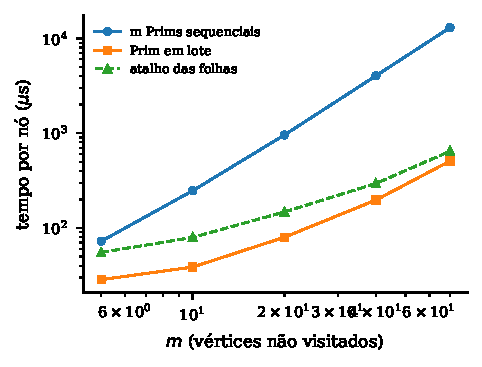
\includegraphics[width=0.5\textwidth]{auditoria_children_mst}
\caption{Tempo para calcular $\mathrm{MST}(R\setminus\{c\})$ para todos os
$m$ filhos de um nó: $m$ execuções sequenciais do Prim, Prim em lote e atalho
das folhas.}\label{fig:auditoria_mst}
\end{figure}

\paragraph{Limites dos filhos no B\&B.} O profiling do B\&B
(Tabela~\ref{tab:perfil}) mostrou que, nas configurações em que a árvore é
grande, 83 a 94\% do tempo vai para o cálculo dos limites dos filhos. Com
Held-Karp e filhos por LB, as árvores são tão pequenas que metade do tempo
vai para o subgradiente na raiz. O Prim em lote foi
25$\times$ mais rápido que $m$ execuções sequenciais em $m=70$ (0,51~ms
contra 12,96~ms). A revisão cruzada sugeriu ainda o \emph{atalho das
folhas}: se $c$ é folha da MST $T$ de $R$, então $T-c$ é MST de $R-c$, e
o limite sai em $O(1)$. A propriedade é verdadeira, e a implementação bate
com o Prim sequencial nos testes. Mesmo assim, ela foi 1,3 a 2,1$\times$
\emph{mais lenta} que o lote para $m\le70$. O atalho exige um Prim extra
com $m$ iterações do interpretador, e nesse tamanho o custo é dominado pelo
número de iterações Python, não pela aritmética, que o NumPy faz em
microssegundos. É um exemplo direto de gargalo teórico que não é o gargalo
prático, por isso a versão em lote continuou como padrão.

\begin{table}[htb]
\centering
\caption{Auditoria dos aproximativos: versão bruta (grafo completo no NetworkX) x refatorada (Prim $O(n^2)$ na matriz, matching só nos vértices ímpares). Tempo: mediana de 3 execuções; memória: pico do tracemalloc.}
\label{tab:auditoria_aprox}
\small
\begin{adjustbox}{max width=\linewidth}
\begin{tabular}{lrlrrrrr}
\toprule
Caso & $N$ & Algoritmo & Tempo bruto (ms) & Tempo ref. (ms) & Speedup & Mem. bruto (MiB) & Mem. ref. (MiB) \\
\midrule
gr24 & 24 & TATT & 0{,}39 & 0{,}08 & 5{,}0$\times$ & 0{,}13 & 0{,}01 \\
gr24 & 24 & Christofides & 1{,}37 & 0{,}66 & 2{,}1$\times$ & 0{,}21 & 0{,}05 \\
att48 & 48 & TATT & 1{,}30 & 0{,}14 & 9{,}0$\times$ & 0{,}46 & 0{,}01 \\
att48 & 48 & Christofides & 9{,}91 & 7{,}02 & 1{,}4$\times$ & 0{,}68 & 0{,}18 \\
st70 & 70 & TATT & 2{,}67 & 0{,}21 & 12{,}7$\times$ & 0{,}90 & 0{,}02 \\
st70 & 70 & Christofides & 11{,}39 & 8{,}08 & 1{,}4$\times$ & 1{,}11 & 0{,}23 \\
random200 & 200 & TATT & 22{,}74 & 0{,}64 & 35{,}5$\times$ & 7{,}78 & 0{,}03 \\
random200 & 200 & Christofides & 155{,}71 & 117{,}47 & 1{,}3$\times$ & 7{,}78 & 1{,}09 \\
random500 & 500 & TATT & 170{,}03 & 1{,}90 & 89{,}4$\times$ & 48{,}94 & 0{,}07 \\
random500 & 500 & Christofides & 2.551{,}72 & 2.221{,}46 & 1{,}1$\times$ & 48{,}94 & 8{,}86 \\
\bottomrule
\end{tabular}
\end{adjustbox}
\end{table}

\begin{table}[htb]
\centering
\caption{Auditoria do B\&B (limite de 30 s por execução; todas as variantes com o mesmo warm-start, vizinho mais próximo, e o mesmo teto de 2 milhões de nós abertos). B/nó aberto: pico de memória dividido pelo máximo de nós abertos, ambos da mesma execução com tracemalloc.}
\label{tab:auditoria_bnb}
\small
\begin{adjustbox}{max width=\linewidth}
\begin{tabular}{llcrrrr}
\toprule
Instância & Variante & Status & Nós exp. & Tempo (s) & Pico (MiB) & B/nó aberto \\
\midrule
burma14 & bruto: best-first, cópias, LB em Python & ótimo & 483.341 & 18{,}13 & 101{,}2 & 259 \\
burma14 & bruto, GC desligado & ótimo & 483.341 & 17{,}78 & 101{,}3 & 260 \\
burma14 & best-first refatorado & ótimo & 237.333 & 3{,}66 & 98{,}1 & 273 \\
burma14 & best-first refatorado, GC desligado & ótimo & 237.333 & 3{,}46 & 98{,}1 & 273 \\
burma14 & DFS, 2 menores arestas & ótimo & 278.533 & 3{,}35 & 0{,}0 & -- \\
burma14 & DFS, 1-árvore & ótimo & 7.772 & 0{,}24 & 0{,}0 & -- \\
burma14 & DFS, Held-Karp & ótimo & 12 & 0{,}00 & 0{,}0 & -- \\
ulysses16 & bruto: best-first, cópias, LB em Python & memória & 337.320 & 27{,}26 & 104{,}0 & 257 \\
ulysses16 & bruto, GC desligado & memória & 337.320 & 25{,}18 & 103{,}9 & 257 \\
ulysses16 & best-first refatorado & memória & 311.106 & 6{,}84 & 365{,}7 & 268 \\
ulysses16 & best-first refatorado, GC desligado & memória & 311.106 & 5{,}75 & 368{,}4 & 268 \\
ulysses16 & DFS, 2 menores arestas & timeout & 2.497.158 & 30{,}00 & 0{,}0 & -- \\
ulysses16 & DFS, 1-árvore & timeout & 1.092.828 & 30{,}00 & 0{,}0 & -- \\
ulysses16 & DFS, Held-Karp & ótimo & 14 & 0{,}01 & 0{,}0 & -- \\
gr17 & bruto: best-first, cópias, LB em Python & timeout & 327.115 & 30{,}42 & 94{,}9 & 260 \\
gr17 & bruto, GC desligado & timeout & 347.969 & 30{,}45 & 95{,}2 & 260 \\
gr17 & best-first refatorado & memória & 419.819 & 8{,}89 & 323{,}4 & 270 \\
gr17 & best-first refatorado, GC desligado & memória & 419.819 & 7{,}72 & 322{,}0 & 270 \\
gr17 & DFS, 2 menores arestas & timeout & 2.426.378 & 30{,}00 & 0{,}0 & -- \\
gr17 & DFS, 1-árvore & ótimo & 293.064 & 10{,}62 & 0{,}0 & -- \\
gr17 & DFS, Held-Karp & ótimo & 15 & 0{,}00 & 0{,}0 & -- \\
\bottomrule
\end{tabular}
\end{adjustbox}
\end{table}


\paragraph{Estratégia da árvore: best-first $\times$ DFS.} Com o mesmo
limite fraco (duas menores arestas), o mesmo warm-start e o mesmo teto de
nós abertos, o best-first refatorado resolveu o burma14 em 3,7~s, contra
18,1~s da versão bruta. Ele expandiu metade dos nós (237 mil contra 483
mil), porque o limite refatorado restringe as arestas livres das pontas do
caminho aos vértices não visitados. Nas duas versões, porém, cada nó aberto
custa cerca de 260 a 270~bytes, e a fila chega a centenas de MiB. No
ulysses16 e no gr17, o best-first estourou o teto de 2 milhões de nós
abertos (320 a 370~MiB) em menos de 10~s. A DFS com o mesmo limite usou
0,03~MiB nas três instâncias. Por isso a DFS é a estratégia padrão: a
memória cai de exponencial para $O(n^2)$, e a perda (expandir nós que o
best-first não expandiria) é compensada por um bom limite. Com Held-Karp, a
DFS resolveu as três instâncias expandindo 12 a 15 nós em menos de 10~ms.
Para o best-first, guardar o caminho como lista encadeada (filho em $O(1)$)
reduziu o custo por nó de $\approx$340 para $\approx$270~bytes. O restante
é o custo fixo de uma tupla Python com 6 campos.


\section{Experimentos e resultados}\label{sec:exp}

\paragraph{Ambiente e protocolo.} Os experimentos rodaram num AMD Ryzen~7
7800X3D (8 núcleos/16 threads, 30~GB), Linux 7.0, Python~3.11.15 e
NumPy~2.4. O limite foi de 30~minutos por execução (heurística mais B\&B);
quem estourou foi registrado como NA, mantendo nós expandidos e podados e o
melhor tour encontrado. A ordem de execução foi:
\begin{enumerate}
  \item as medições sensíveis a tempo (heurísticas, escala e auditoria),
    rodadas \emph{uma de cada vez}, com a máquina sem outra carga;
  \item o B\&B com Held-Karp na TSPLIB, com 4 processos em paralelo;
  \item a escala do B\&B e as instâncias sintéticas, cujas métricas
    principais (nós e custo) não dependem da máquina.
\end{enumerate}
O B\&B com 1-árvore veio de um primeiro lote com 8 processos e não foi
refeito: o código da DFS não mudou, e quase metade dessas 150 execuções
estoura o limite. Nesse lote, árvores idênticas chegaram a levar
2$\times$ mais tempo, então a métrica principal do B\&B é o número de nós.
Todas as 309 execuções do B\&B que terminaram (incluindo as 75 com o GC
desligado) reproduziram o ótimo publicado.

\subsection{Complexidade empírica}\label{sec:complexidade}

Na TSPLIB, $N\in[14,70]$ é estreito demais para distinguir $n^2$ de $n^3$.
Por isso as curvas foram ajustadas em instâncias uniformes no quadrado
$[0,10^4]^2$ (distância EUC\_2D), com $N$ de 25 a 6400 (o blossom só até
1000) e 3 sementes por $N$. A Tabela~\ref{tab:complexidade} traz, para cada
subrotina, duas coisas:
\begin{itemize}
  \item o expoente livre $b$ de $t=aN^b$, ajustado em log-log;
  \item o ajuste do modelo teórico $t=c_0+c_1f(N)$ na escala original, com
    $R^2$ e RMSE, como pede o enunciado.
\end{itemize}

\begin{table}[htb]
\centering
\caption{Ajuste do tempo em função de $N$ (medianas de 3 sementes, $N=25$ a $6400$; blossom até $1000$). $b$: expoente da lei de potência $t=aN^b$ (log-log). Melhor forma: modelo teórico com menor RMSE em escala log. $R^2$/RMSE teoria: ajuste $t=c_0+c_1f(N)$ do modelo teórico em escala linear.}
\label{tab:complexidade}
\small
\begin{adjustbox}{max width=\linewidth}
\begin{tabular}{llcccccc}
\toprule
Algoritmo & Subrotina & Teoria & $b$ (IC 95\%) & $R^2_{\log}$ & Melhor forma & $R^2$ teoria & RMSE (ms) \\
\midrule
Viz. próximo & total & $n^2$ & 1{,}20 $\pm$ 0{,}11 & 0{,}988 & $n\log n$ & 0{,}995 & 0{,}889 \\
Fecho convexo & total & $n^2$ & 1{,}55 $\pm$ 0{,}17 & 0{,}981 & $n\log n$ & 0{,}996 & 42{,}363 \\
TATT & total & $n^2$ & 1{,}20 $\pm$ 0{,}08 & 0{,}993 & $n\log n$ & 0{,}989 & 2{,}113 \\
TATT & MST (Prim) & $n^2$ & 1{,}22 $\pm$ 0{,}08 & 0{,}994 & $n\log n$ & 0{,}990 & 1{,}982 \\
TATT & pré-ordem & $n$ & 0{,}99 $\pm$ 0{,}06 & 0{,}995 & $n$ & 0{,}995 & 0{,}043 \\
Christofides (blossom) & total & $n^3$ & 2{,}81 $\pm$ 0{,}20 & 0{,}996 & $n^3$ & 0{,}997 & 331{,}478 \\
Christofides (blossom) & MST (Prim) & $n^2$ & 1{,}13 $\pm$ 0{,}07 & 0{,}997 & $n\log n$ & 0{,}980 & 0{,}239 \\
Christofides (blossom) & vértices ímpares & $n$ & 0{,}31 $\pm$ 0{,}10 & 0{,}926 & $n$ & 0{,}915 & 0{,}002 \\
Christofides (blossom) & matching: grafo & $n^2$ & 1{,}78 $\pm$ 0{,}27 & 0{,}983 & $n^2$ & 0{,}996 & 0{,}920 \\
Christofides (blossom) & matching: blossom & $n^3$ & 2{,}89 $\pm$ 0{,}15 & 0{,}998 & $n^3$ & 0{,}997 & 333{,}007 \\
Christofides (blossom) & Hierholzer & $n$ & 1{,}01 $\pm$ 0{,}06 & 0{,}997 & $n$ & 0{,}996 & 0{,}018 \\
Christofides (blossom) & atalhos & $n$ & 0{,}82 $\pm$ 0{,}07 & 0{,}994 & $n$ & 0{,}999 & 0{,}000 \\
Christofides (guloso) & total & $n^2\log n$ & 1{,}52 $\pm$ 0{,}20 & 0{,}975 & $n\log n$ & 1{,}000 & 0{,}971 \\
Christofides (guloso) & MST (Prim) & -- & 1{,}23 $\pm$ 0{,}08 & 0{,}993 & $n\log n$ & -- & -- \\
Christofides (guloso) & vértices ímpares & -- & 0{,}32 $\pm$ 0{,}12 & 0{,}828 & $n$ & -- & -- \\
Christofides (guloso) & matching: blossom & $n^2\log n$ & 1{,}82 $\pm$ 0{,}23 & 0{,}977 & $n^2$ & 1{,}000 & 3{,}247 \\
Christofides (guloso) & Hierholzer & -- & 1{,}04 $\pm$ 0{,}03 & 0{,}998 & $n$ & -- & -- \\
Christofides (guloso) & atalhos & -- & 0{,}89 $\pm$ 0{,}06 & 0{,}994 & $n$ & -- & -- \\
\bottomrule
\end{tabular}
\end{adjustbox}
\end{table}


\begin{figure}[htb]
\centering
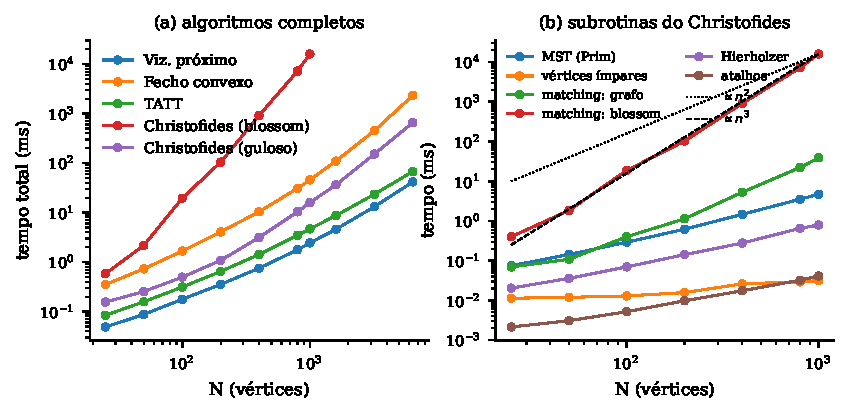
\includegraphics[width=\textwidth]{tempo_vs_n}
\caption{Tempo em função de $N$ (medianas). (a) Algoritmos completos. (b)
Subrotinas do Christofides com retas de referência $\propto n^2$ e
$\propto n^3$.}\label{fig:tempo}
\end{figure}

\paragraph{Onde a teoria aparece.} O blossom segue a teoria com precisão:
$b=2{,}89\pm0{,}15$, contra $O(k^3)$, com $R^2=0{,}997$ para
$c_0+c_1N^3$. Como ele domina, o Christofides inteiro também cresce como
$N^{2{,}81}$. A construção do grafo do matching cresce como $N^{1{,}78}$
($O(k^2)$ arestas), e Hierholzer e pré-ordem são lineares ($b\approx1$).
O matching guloso fica em $N^{1{,}82}$, próximo de $O(k^2\log k)$.

\paragraph{Onde a teoria não aparece.} Prim e vizinho mais próximo são
$O(n^2)$, mas os expoentes medidos foram 1,22 e 1,20. Os dois têm $n$
iterações, cada uma com uma operação NumPy de tamanho $n$. Para $n$ de
milhares, o vetor (até 50~KB) cabe na cache, e a operação vetorizada custa
poucos nanossegundos por elemento, contra microssegundos fixos do
interpretador por iteração. O termo $O(n)$ por iteração só passa a dominar
com $N$ grande: o expoente \emph{local} do Prim, entre $N$ e $2N$, sobe de
0,97 ($N\le100$) para 1,54 (3200 a 6400), e o do vizinho mais próximo de
0,84 para 1,66. A inserção a partir do fecho convexo passa de 2 no fim
(2,37 entre 3200 e 6400), pelos recálculos das inserções invalidadas. Nesse
regime, o modelo teórico ajusta bem na escala linear ($R^2\ge0{,}98$), mas
$n\log n$ descreve melhor a \emph{forma} da curva: até $N\approx10^3$, o
custo prático de um algoritmo $O(n^2)$ vetorizado é dominado pelo número
de iterações do interpretador.

\paragraph{Memória.} A Tabela~\ref{tab:memoria} confirma $O(n^2)$ na
construção do grafo do matching ($b=2{,}01$, 36~MiB em $N=1000$, contra
31~KiB da MST). No matching guloso a memória também é $O(n^2)$ ($b=2{,}03$,
438~MiB em $N=6400$), por causa dos vetores de índices de todos os $k^2/2$
pares. As subrotinas lineares ficam com $b<1$ para $N$ pequeno porque há um
custo fixo de alocação.

\begin{table}[htb]
\centering
\caption{Expoente do pico de memória extra (tracemalloc) em função de $N$.}
\label{tab:memoria}
\small
\begin{adjustbox}{max width=\linewidth}
\begin{tabular}{llcccr}
\toprule
Algoritmo & Subrotina & Teoria & $b$ (IC 95\%) & $R^2_{\log}$ & Pico em $N_{\max}$ (KiB) \\
\midrule
Viz. próximo & total & $n$ & 0{,}75 $\pm$ 0{,}09 & 0{,}977 & 463{,}0 \\
Fecho convexo & total & $n$ & 1{,}32 $\pm$ 0{,}12 & 0{,}989 & 18.257{,}6 \\
TATT & total & $n$ & 0{,}92 $\pm$ 0{,}08 & 0{,}990 & 853{,}3 \\
TATT & MST (Prim) & $n$ & 0{,}55 $\pm$ 0{,}08 & 0{,}968 & 146{,}9 \\
TATT & pré-ordem & -- & 1{,}04 $\pm$ 0{,}03 & 0{,}999 & 802{,}1 \\
Christofides (blossom) & total & $n^2$ & 1{,}87 $\pm$ 0{,}18 & 0{,}993 & 36.358{,}4 \\
Christofides (blossom) & MST (Prim) & $n$ & 0{,}46 $\pm$ 0{,}08 & 0{,}977 & 31{,}5 \\
Christofides (blossom) & vértices ímpares & -- & 0{,}36 $\pm$ 0{,}12 & 0{,}925 & 22{,}3 \\
Christofides (blossom) & matching: grafo & $n^2$ & 2{,}01 $\pm$ 0{,}13 & 0{,}997 & 36.345{,}5 \\
Christofides (blossom) & matching: blossom & $n^2$ & 1{,}07 $\pm$ 0{,}20 & 0{,}975 & 827{,}3 \\
Christofides (blossom) & Hierholzer & -- & 1{,}05 $\pm$ 0{,}04 & 0{,}999 & 386{,}7 \\
Christofides (blossom) & atalhos & -- & 0{,}62 $\pm$ 0{,}16 & 0{,}953 & 9{,}9 \\
Christofides (guloso) & total & $n^2$ & 2{,}00 $\pm$ 0{,}16 & 0{,}990 & 448.597{,}2 \\
Christofides (guloso) & MST (Prim) & -- & 0{,}55 $\pm$ 0{,}08 & 0{,}968 & 146{,}9 \\
Christofides (guloso) & vértices ímpares & -- & 0{,}52 $\pm$ 0{,}13 & 0{,}919 & 112{,}0 \\
Christofides (guloso) & matching: blossom & -- & 2{,}03 $\pm$ 0{,}15 & 0{,}992 & 448.524{,}2 \\
Christofides (guloso) & Hierholzer & -- & 1{,}05 $\pm$ 0{,}02 & 0{,}999 & 2.584{,}7 \\
Christofides (guloso) & atalhos & -- & 0{,}84 $\pm$ 0{,}08 & 0{,}987 & 58{,}4 \\
\bottomrule
\end{tabular}
\end{adjustbox}
\end{table}


\paragraph{Garbage collection.} Toda a escala foi repetida com o GC
desligado (Tabela~\ref{tab:gc}). O Christofides chega a 194 coletas por
execução em $N=1000$, porque o NetworkX cria milhões de objetos Python.
Mesmo assim, a razão entre os tempos com e sem GC ficou entre 0,95 e 1,06
(mediana 1,01), e nenhum expoente mudou mais que 0,02. No B\&B em DFS, a
mediana foi de 0 coletas por execução, e o tempo de CPU com e sem GC
diferiu menos de 2\%. O GC \emph{não} distorce a complexidade aqui.
\begin{itemize}
  \item Os dados grandes vivem em vetores NumPy, que não são rastreados
    pelo GC.
  \item O que cria muitos objetos pequenos é o best-first. Na auditoria,
    desligar o GC aumentou a vazão dele em 2 a 19\%.
  \item As distorções de memória que pesaram foram \emph{cópias}: a cópia
    da matriz inteira no vizinho mais próximo (7,7~MiB em $N=1000$,
    removida) e o grafo completo do NetworkX (49~MiB em $N=500$).
\end{itemize}

\begin{table}[htb]
\centering
\caption{Expoente do tempo total com e sem o coletor de lixo.}
\label{tab:gc}
\small
\begin{adjustbox}{max width=\linewidth}
\begin{tabular}{lcc}
\toprule
Algoritmo & $b$ com GC & $b$ sem GC \\
\midrule
Christofides (blossom) & 2{,}81 & 2{,}80 \\
Christofides (guloso) & 1{,}52 & 1{,}51 \\
Fecho convexo & 1{,}55 & 1{,}54 \\
Viz. próximo & 1{,}20 & 1{,}19 \\
TATT & 1{,}20 & 1{,}19 \\
\bottomrule
\end{tabular}
\end{adjustbox}
\end{table}


\paragraph{Crescimento do B\&B.} Com 10 sementes por $N$ em instâncias
uniformes (Tabela~\ref{tab:bnbescala}, Figura~\ref{fig:bnbescala}), o
número de nós da 1-árvore cresce exponencialmente: cada vértice a mais
multiplica a árvore por 1,54 ($R^2=0{,}986$ no modelo exponencial, contra
0,952 no polinomial). O Held-Karp é tão apertado em pontos uniformes que,
até $N=30$, a DFS desce direto ao ótimo (exatamente $N-2$ nós expandidos).
O crescimento só aparece de $N=35$ em diante e varia muito entre sementes
(fator ajustado de 1,22, $R^2=0{,}88$). O tempo por nó cresce só como
$N^{0{,}65\text{--}0{,}76}$, apesar de ser $O(m^3)$ por nó. É o mesmo
efeito do interpretador visto acima: o Prim em lote tem $m$ iterações
Python, e a aritmética de cada uma é barata. A memória da DFS ficou em
140~KiB com $N=50$.

\begin{table}[htb]
\centering
\caption{Crescimento do B\&B (DFS, filhos por limite, warm-start vizinho mais próximo) em instâncias uniformes. Fator/vértice: $10^{\beta}$ do ajuste $\log_{10}(\text{nós}) = \alpha + \beta N$. $b$ tempo/nó: expoente do tempo de cálculo dos limites por nó expandido; $b$ memória: expoente do pico de memória (tracemalloc) em função de $N$.}
\label{tab:bnbescala}
\small
\begin{adjustbox}{max width=\linewidth}
\begin{tabular}{lcrccccc}
\toprule
Limite & $N$ & Timeouts & Fator/vértice & $R^2$ exp. & $R^2$ polin. & $b$ tempo/nó & $b$ memória \\
\midrule
Held-Karp & 10--50 & 0 & 1{,}21 & 0{,}882 & 0{,}752 & 0{,}65 & 1{,}06 \\
1-árvore & 8--26 & 0 & 1{,}54 & 0{,}986 & 0{,}952 & 0{,}76 & 0{,}88 \\
\bottomrule
\end{tabular}
\end{adjustbox}
\end{table}


\begin{figure}[htb]
\centering
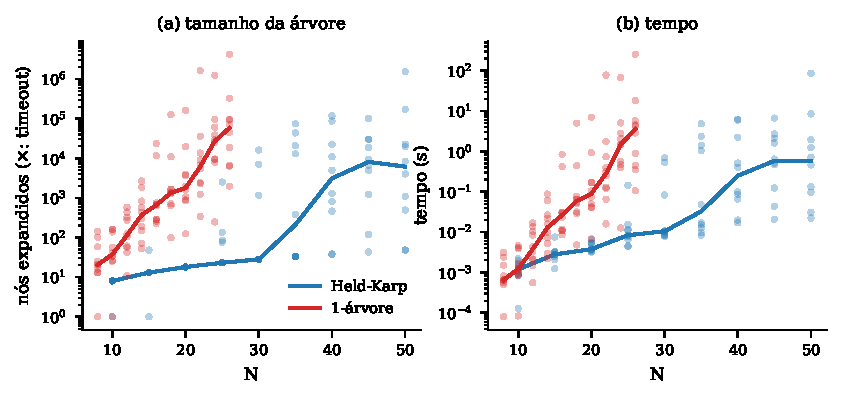
\includegraphics[width=\textwidth]{bnb_escala}
\caption{B\&B (DFS, filhos por LB) em instâncias uniformes, 10 sementes por
$N$; linhas = mediana.}\label{fig:bnbescala}
\end{figure}

\subsection{Impacto do warm-start na árvore de busca}\label{sec:warmstart}

Foram 300 execuções: 15 instâncias $\times$ 5 warm-starts $\times$ 4
configurações. As configurações combinam o limite (Held-Karp ou 1-árvore)
com a ordem dos filhos na DFS (por LB ou por índice). A
Tabela~\ref{tab:warmstart} resume os resultados, e a
Figura~\ref{fig:heatmap} mostra os nós expandidos de cada execução.

\begin{table}[htb]
\centering
\caption{Impacto do warm-start no B\&B (DFS, 15 instâncias, limite de 30 min). Nós exp. (geo): média geométrica dos nós expandidos nas instâncias que todas as estratégias resolveram; razão vs trivial: média geométrica da razão por instância. Posto tempo: posto médio do tempo total (timeout = 1800 s; 1 = mais rápido). Tempo total: soma das 15 execuções.}
\label{tab:warmstart}
\small
\setlength{\tabcolsep}{4pt}
\begin{adjustbox}{max width=\linewidth}
\begin{tabular}{llcrrrrr}
\toprule
Configuração & Warm-start & Resolv. & Gap inicial & Nós exp. (geo) & Razão vs trivial & Posto tempo & Tempo total (s) \\
\midrule
Held-Karp, filhos por LB & Trivial & 15/15 & 152{,}3\% & 193 & 1{,}000 & 2{,}20 & 76 \\
 & Viz. próximo & 15/15 & 24{,}8\% & 244 & 1{,}260 & 2{,}40 & 76 \\
 & Fecho convexo & 15/15 & 2{,}5\% & 129 & 0{,}669 & 2{,}53 & 38 \\
 & TATT & 15/15 & 28{,}5\% & 243 & 1{,}260 & 3{,}07 & 77 \\
 & Christofides & 15/15 & 8{,}1\% & 209 & 1{,}083 & 4{,}80 & 76 \\
\midrule
Held-Karp, filhos por índice & Trivial & 13/15 & 152{,}3\% & 9.236 & 1{,}000 & 4{,}53 & 5.464 \\
 & Viz. próximo & 15/15 & 24{,}8\% & 2.918 & 0{,}316 & 2{,}87 & 1.213 \\
 & Fecho convexo & 15/15 & 2{,}5\% & 224 & 0{,}024 & 1{,}20 & 102 \\
 & TATT & 15/15 & 28{,}5\% & 3.788 & 0{,}410 & 3{,}73 & 2.061 \\
 & Christofides & 15/15 & 8{,}1\% & 1.256 & 0{,}136 & 2{,}67 & 787 \\
\midrule
1-árvore, filhos por LB & Trivial & 9/15 & 152{,}3\% & 384.143 & 1{,}000 & 2{,}80 & 12.886 \\
 & Viz. próximo & 9/15 & 24{,}8\% & 386.606 & 1{,}006 & 3{,}47 & 12.959 \\
 & Fecho convexo & 9/15 & 2{,}5\% & 361.217 & 0{,}940 & 2{,}33 & 12.894 \\
 & TATT & 9/15 & 28{,}5\% & 386.644 & 1{,}007 & 3{,}20 & 12.937 \\
 & Christofides & 9/15 & 8{,}1\% & 385.704 & 1{,}004 & 3{,}20 & 12.942 \\
\midrule
1-árvore, filhos por índice & Trivial & 8/15 & 152{,}3\% & 524.360 & 1{,}000 & 3{,}83 & 14.244 \\
 & Viz. próximo & 8/15 & 24{,}8\% & 429.894 & 0{,}820 & 3{,}30 & 14.225 \\
 & Fecho convexo & 9/15 & 2{,}5\% & 261.998 & 0{,}500 & 2{,}20 & 13.427 \\
 & TATT & 8/15 & 28{,}5\% & 457.197 & 0{,}872 & 3{,}03 & 14.190 \\
 & Christofides & 8/15 & 8{,}1\% & 344.515 & 0{,}657 & 2{,}63 & 14.063 \\
\bottomrule
\end{tabular}
\end{adjustbox}
\end{table}


\begin{figure}[htb]
\centering
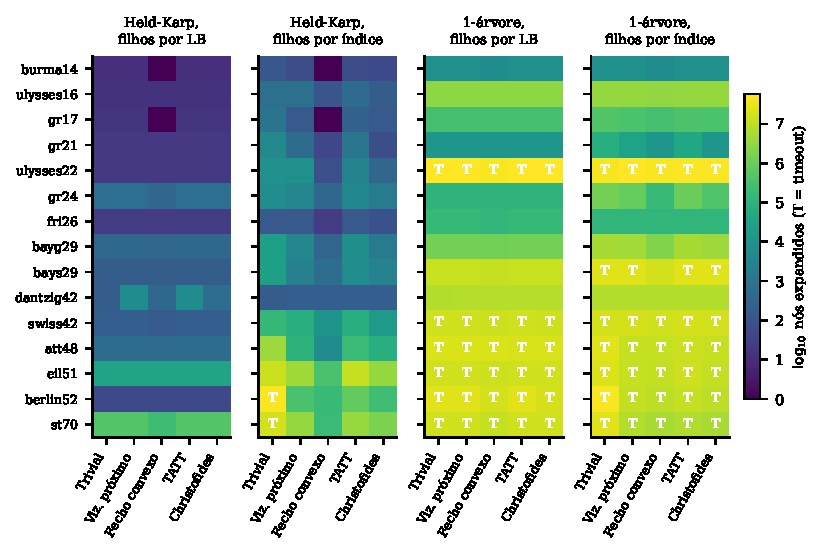
\includegraphics[width=\textwidth]{warmstart_heatmap}
\caption{Nós expandidos ($\log_{10}$) por instância, estratégia e
configuração. T: estourou 30 minutos.}\label{fig:heatmap}
\end{figure}

\paragraph{Quando o warm-start importa.} Com filhos visitados por índice, a
DFS não tem guia: no começo, a única fonte de poda é a incumbente. Nesse
regime a qualidade do limite superior inicial decide o tamanho da árvore.
Com Held-Karp e filhos por índice:
\begin{itemize}
  \item a solução trivial (gap inicial médio de 152\%) deixou berlin52 e
    st70 sem terminar em 30~minutos;
  \item todas as heurísticas resolveram as 15 instâncias;
  \item a inserção a partir do fecho convexo (gap médio de 2,5\%) expandiu
    em média 41$\times$ menos nós que a trivial (razão geométrica 0,024), o
    Christofides 7$\times$ menos (0,136), o vizinho mais próximo 3$\times$
    e o TATT 2,4$\times$.
\end{itemize}
O tempo total das 15 execuções caiu de 5464~s (trivial) para 102~s (fecho).
Dentro de cada instância, o número de nós acompanha o gap inicial
(correlação de Spearman média de 0,97). Os perfis por profundidade
(Figura~\ref{fig:profundidade}) mostram o mecanismo: com um UB bom, a poda
começa nos níveis rasos, e a árvore nem chega a abrir os ramos ruins.

\paragraph{Quando quase não importa.} Com filhos ordenados por LB, a
primeira descida da DFS já se comporta como uma heurística gulosa guiada
pelo limite. Com Held-Karp ela encontra um tour ótimo ou quase ótimo em
milissegundos, e o UB inicial deixa de ser a fonte principal de poda.
\begin{itemize}
  \item As 15 instâncias foram resolvidas com qualquer warm-start, e as
    razões de nós ficaram entre 0,67 (fecho) e 1,26.
  \item Um UB inicial melhor pode até \emph{aumentar} a árvore. No
    dantzig42, a solução trivial é ótima (699) e levou a 190 nós; o vizinho
    mais próximo levou a 6078. A diferença está no desempate: com outra
    incumbente, a primeira descida segue outro ramo de mesmo LB.
\end{itemize}
Com a 1-árvore, os dois regimes se confundem. O limite é tão fraco (gap de
10 a 31\% na raiz) que as árvores têm milhões de nós de qualquer forma. As
razões ficam entre 0,94 e 1,01 com filhos por LB, e entre 0,50 e 0,87 com
filhos por índice. O teste de Friedman (Tabela~\ref{tab:friedman}) não
rejeita a igualdade do tempo entre as estratégias com 1-árvore e filhos por
LB ($p=0{,}10$), e rejeita com folga nas configurações em que o UB
importa.

\begin{figure}[htb]
\centering
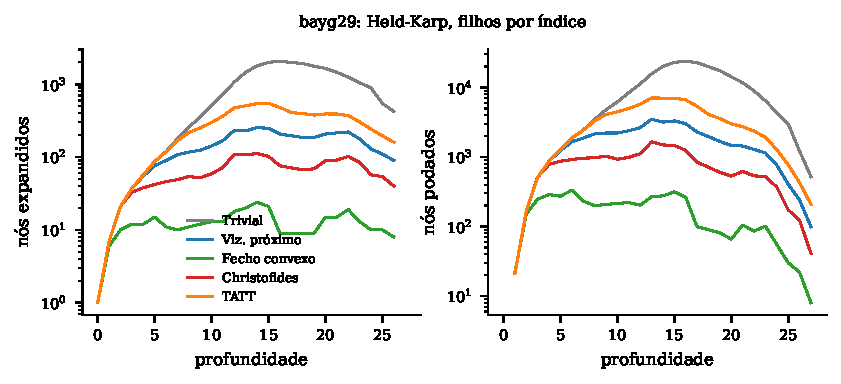
\includegraphics[width=\textwidth]{warmstart_profundidade_bayg29}
\caption{Nós expandidos e podados por profundidade, bayg29 (Held-Karp,
filhos por índice).}\label{fig:profundidade}
\end{figure}

\begin{table}[htb]
\centering
\caption{Teste de Friedman (4 graus de liberdade) para a hipótese de que as cinco estratégias de warm-start têm o mesmo desempenho.}
\label{tab:friedman}
\small
\begin{adjustbox}{max width=\linewidth}
\begin{tabular}{lcccc}
\toprule
Configuração & $\chi^2_F$ tempo & $p$ tempo & $\chi^2_F$ nós & $p$ nós \\
\midrule
Held-Karp, filhos por LB & 26{,}8 & 2{,}2e-05 & 25{,}8 & 3{,}5e-05 \\
Held-Karp, filhos por índice & 37{,}5 & 1{,}4e-07 & 38{,}3 & 9{,}6e-08 \\
1-árvore, filhos por LB & 7{,}8 & 9{,}8e-02 & 26{,}0 & 3{,}1e-05 \\
1-árvore, filhos por índice & 16{,}5 & 2{,}4e-03 & 24{,}1 & 7{,}6e-05 \\
\bottomrule
\end{tabular}
\end{adjustbox}
\end{table}


\paragraph{O tempo da heurística compensa?} Sim, sempre que o UB importa.
As heurísticas levaram de 0,08~ms (vizinho mais próximo) a 1,7~ms
(Christofides, mediana), e no máximo 8,8~ms. Com Held-Karp e filhos por
índice, a economia de tempo superou o custo da heurística em 13 a 14 das 15
instâncias, num total de 3400 a 5360~s economizados contra menos de 0,04~s
gastos. Com filhos por LB, o B\&B inteiro leva dezenas de milissegundos nas
instâncias pequenas. Aí os 1,7~ms do Christofides chegam a pesar mais que a
busca, e ele ficou com o pior posto médio de tempo (4,8). O vizinho mais
próximo é o que melhor equilibra custo e qualidade quando não se sabe a
ordem dos filhos; o fecho convexo é o melhor em qualidade a um custo ainda
desprezível (0,5~ms).

\paragraph{Ponto de colapso.} A Tabela~\ref{tab:colapso} mostra onde o
B\&B exato deixa de terminar em 30~minutos. Com Held-Karp e filhos por LB,
todas as 15 instâncias foram resolvidas, até o st70, em no máximo 72~s. Com
filhos por índice, o primeiro timeout foi em $N=52$ (berlin52, só com a
trivial). Com a 1-árvore, o colapso começa em $N=22$ (ulysses22), e
nenhuma instância com $N\ge48$ terminou. Entre 22 e 42, ele depende da
instância: dantzig42 terminou, swiss42 não. Mesmo nesses casos, os
aproximativos rodam em milissegundos (Seção~\ref{sec:complexidade}).

\begin{table}[htb]
\centering
\caption{Ponto de colapso do B\&B exato na TSPLIB (30 min).}
\label{tab:colapso}
\small
\begin{adjustbox}{max width=\linewidth}
\begin{tabular}{lcccc}
\toprule
Configuração & Resolvidas (alguma) & Resolvidas (todas) & Maior $N$ resolvido & Menor $N$ com timeout \\
\midrule
Held-Karp, filhos por LB & 15/15 & 15/15 & 70 & -- \\
Held-Karp, filhos por índice & 15/15 & 13/15 & 70 & 52 \\
1-árvore, filhos por LB & 9/15 & 9/15 & 42 & 22 \\
1-árvore, filhos por índice & 9/15 & 8/15 & 42 & 22 \\
\bottomrule
\end{tabular}
\end{adjustbox}
\end{table}

\begin{table}[htb]
\centering
\caption{Profiling do B\&B: mediana, nas 75 execuções de cada configuração, da fração do tempo total em cada subrotina, e tempo de cálculo dos limites por nó expandido. O restante é a própria busca (recursão, ordenação).}
\label{tab:perfil}
\small
\begin{adjustbox}{max width=\linewidth}
\begin{tabular}{lrrrr}
\toprule
Configuração & Heurística & Limite na raiz & Limites dos filhos & $\mu$s por nó \\
\midrule
Held-Karp, filhos por LB & 0{,}75\% & 50{,}9\% & 44{,}8\% & 59 \\
Held-Karp, filhos por índice & 0{,}08\% & 6{,}7\% & 83{,}0\% & 48 \\
1-árvore, filhos por LB & 0{,}00\% & 0{,}0\% & 94{,}4\% & 67 \\
1-árvore, filhos por índice & 0{,}00\% & 0{,}0\% & 90{,}7\% & 68 \\
\bottomrule
\end{tabular}
\end{adjustbox}
\end{table}


\subsection{Sensibilidade às características das instâncias}\label{sec:sens}

Quinze instâncias são poucas para um modelo com 13 features. Geramos então
168 instâncias sintéticas \emph{adversariais}, com $N\in\{20,30,40,50\}$ e 6
sementes, em sete famílias. Cada família estressa uma feature pedida:
\begin{itemize}
  \item \emph{uniforme}: a referência;
  \item \emph{aglomerados}: silhueta alta e Clark-Evans $<1$;
  \item \emph{grade}: Clark-Evans $>1$ e muitos empates no vizinho mais
    próximo;
  \item \emph{anel}: quase todos os pontos no fecho;
  \item \emph{faixa}: razão de aspecto entre 0,05 e 0,2;
  \item \emph{núcleo denso e pontos dispersos}: alto CV da distância ao
    vizinho mais próximo;
  \item \emph{raios}: hubs na MST.
\end{itemize}
O ótimo exato de cada uma veio do B\&B com Held-Karp, com limite de 15~min;
159 das 168 foram resolvidas, e o gap de cada heurística é exato. O
índice de Clark-Evans~\cite{clarkevans1954} usa a correção de borda de
Donnelly~\cite{donnelly1978}. Sem ela, com $N$ pequeno, todas as 15
instâncias da TSPLIB davam $>1$, até as claramente agrupadas. A base final
tem 174 instâncias, e os modelos são avaliados por validação cruzada
(5 partes, 10 repetições).

\begin{table}[htb]
\centering
\caption{Mediana do gap (\%) por família de instância. A última coluna é o gap do limite de 1-árvore na raiz do B\&B.}
\label{tab:familias}
\small
\begin{adjustbox}{max width=\linewidth}
\begin{tabular}{lrrrrrrr}
\toprule
Família & Inst. & Viz. próximo & Fecho convexo & TATT & Christofides & Christ. guloso & gap raiz 1-árvore \\
\midrule
uniforme & 24 & 20{,}1 & 3{,}3 & 35{,}4 & 10{,}4 & 13{,}6 & 11{,}9 \\
aglomerados & 18 & 16{,}4 & 1{,}2 & 19{,}2 & 6{,}8 & 11{,}9 & 27{,}1 \\
grade & 24 & 27{,}2 & 5{,}3 & 32{,}8 & 13{,}2 & 20{,}5 & 5{,}4 \\
anel & 24 & 0{,}0 & 0{,}0 & 23{,}0 & 0{,}0 & 0{,}0 & 5{,}8 \\
faixa & 22 & 18{,}7 & 0{,}1 & 15{,}6 & 9{,}6 & 18{,}9 & 25{,}5 \\
núcleo+dispersos & 23 & 16{,}5 & 2{,}9 & 17{,}0 & 7{,}3 & 13{,}2 & 28{,}2 \\
raios & 24 & 18{,}2 & 2{,}5 & 25{,}2 & 8{,}8 & 13{,}5 & 26{,}8 \\
TSPLIB & 15 & 22{,}1 & 2{,}2 & 31{,}0 & 7{,}5 & 17{,}2 & 15{,}0 \\
\bottomrule
\end{tabular}
\end{adjustbox}
\end{table}


\paragraph{Instâncias adversariais.} Cada família estressa as heurísticas
de um jeito (Tabela~\ref{tab:familias}, Figura~\ref{fig:familias}):
\begin{itemize}
  \item \emph{Grade} é a pior para quase todas: o vizinho mais próximo
    chega a 27\% de gap, e o Christofides a 13\%. Com distâncias quase
    iguais, as escolhas locais empatam, e os desempates errados se acumulam.
  \item \emph{Anel} é trivial para todas as heurísticas, menos o TATT (23\%
    de gap): a MST de pontos num círculo é um caminho, e a pré-ordem a
    percorre bem, mas a aresta de volta atravessa o anel.
  \item Para o limite de 1-árvore, as piores são as estruturadas:
    aglomerados, núcleo com dispersos, faixa e raios, todas com 25 a 28\%
    de gap na raiz, contra 12\% na uniforme e 5\% na grade. A MST liga os
    grupos com poucas arestas longas e tem muitas folhas, então fica longe
    de um caminho hamiltoniano.
\end{itemize}
O Held-Karp corrige os graus com as penalidades $\pi$ e fechou essa
diferença: mediana de 0 a 0,2\% em todas as famílias.

\begin{figure}[htb]
\centering
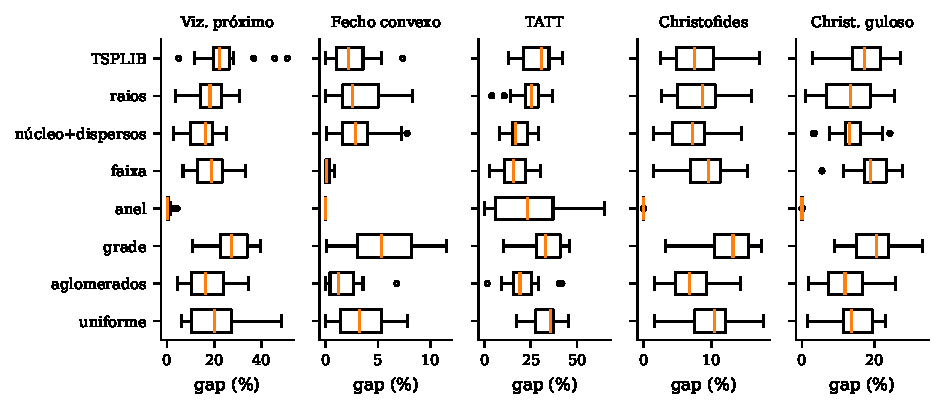
\includegraphics[width=\textwidth]{sensibilidade_familias}
\caption{Gap por família (instâncias sintéticas com ótimo exato e TSPLIB).}\label{fig:familias}
\end{figure}

\begin{figure}[htb]
\centering
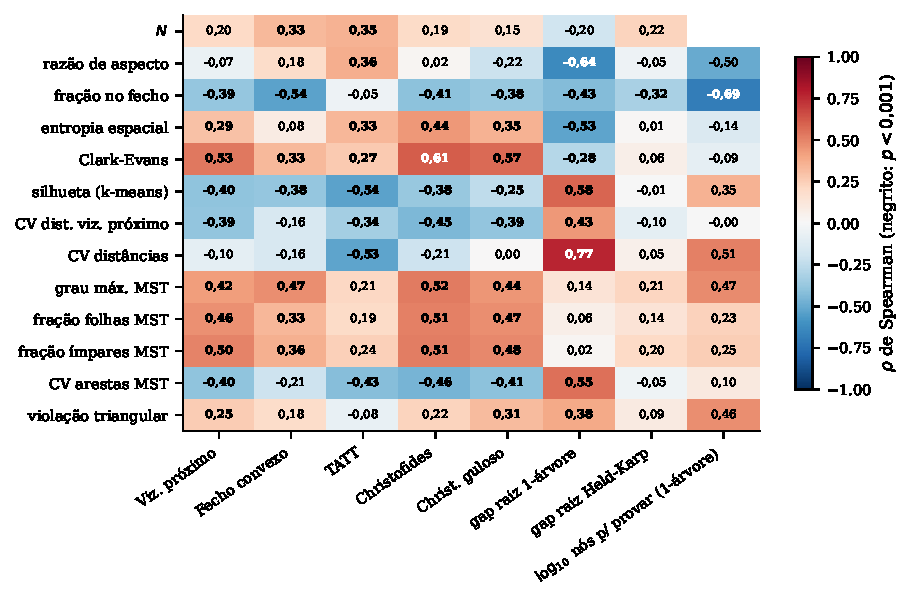
\includegraphics[width=0.95\textwidth]{sensibilidade_spearman}
\caption{Correlação de Spearman entre features e gaps nas 174 instâncias.}\label{fig:spearman}
\end{figure}

\paragraph{Peso das features.} A Figura~\ref{fig:spearman} mostra as
correlações. Para os modelos, três features com VIF $>10$ foram removidas
(fração de folhas da MST, CV das arestas da MST e CV das distâncias).
Sobraram 10 features padronizadas para a regressão múltipla
(Tabela~\ref{tab:coeficientes}), a árvore de decisão de profundidade 3
(Figura~\ref{fig:arvore}) e a floresta aleatória~\cite{breiman2001}.
\begin{itemize}
  \item \emph{Fração de pontos no fecho convexo.} É a feature mais forte e
    consistente: um desvio padrão a mais reduz o gap do Christofides em
    2,2 pontos percentuais e o do vizinho mais próximo em 2,5. Ela também é
    a primeira divisão das árvores. Com mais de 47\% dos pontos no fecho,
    o gap médio do Christofides fica abaixo de 0,5\%.
  \item \emph{Clark-Evans e entropia espacial} pioram o Christofides
    ($+2{,}1$ cada, $p<0{,}001$). Pontos regulares e espalhados são o caso
    difícil, como na família grade.
  \item \emph{Fração de vértices ímpares na MST} pesa no vizinho mais
    próximo e no TATT ($+3{,}5$ e $+4{,}6$). Ela é proporcional ao tamanho
    do matching e mede quanto a MST se ramifica. O grau máximo da MST
    (hubs) tem efeito pequeno: $+0{,}7$ no Christofides, $p=0{,}02$.
  \item \emph{O gap do limite de 1-árvore na raiz} é o mais previsível
    ($R^2_{CV}=0{,}83$). Ele cai com a fração no fecho ($-6{,}9$), com $N$
    e com Clark-Evans, ou seja, é maior em instâncias agrupadas.
\end{itemize}
Os gaps das heurísticas são explicados só em parte: o $R^2_{CV}$ fica entre
0,30 (TATT) e 0,58 (Christofides). O resto depende de detalhes
combinatórios, como empates e a ordem dos vértices, que as features globais
não capturam. A árvore de decisão sozinha generaliza pior que a regressão
(Tabela~\ref{tab:modelos}), mas suas regras são legíveis e coincidem com
os coeficientes.

\begin{table}[htb]
\centering
\caption{Coeficientes padronizados da regressão múltipla (variação do gap, em pontos percentuais, por desvio padrão da feature). $^{*}p<0{,}05$, $^{**}p<0{,}01$, $^{***}p<0{,}001$.}
\label{tab:coeficientes}
\small
\begin{adjustbox}{max width=\linewidth}
\begin{tabular}{lrrrrrr}
\toprule
Feature & Viz. próximo & Fecho convexo & TATT & Christofides & Christ. guloso & gap raiz 1-árvore \\
\midrule
$N$ & 1{,}07 & 0{,}39$^{*}$ & 4{,}09$^{***}$ & 0{,}14 & 0{,}82 & -3{,}91$^{***}$ \\
razão de aspecto & -1{,}70 & 0{,}71$^{**}$ & 2{,}75$^{**}$ & 1{,}01$^{**}$ & -1{,}23$^{*}$ & -3{,}53$^{***}$ \\
fração no fecho & -2{,}45$^{*}$ & -0{,}74$^{**}$ & 2{,}30 & -2{,}20$^{***}$ & -2{,}90$^{***}$ & -6{,}91$^{***}$ \\
entropia espacial & 0{,}02 & -0{,}55 & 1{,}19 & 2{,}15$^{***}$ & 1{,}57 & -2{,}00$^{**}$ \\
Clark-Evans & 0{,}90 & 1{,}03$^{**}$ & -2{,}24 & 2{,}14$^{***}$ & 2{,}93$^{**}$ & -3{,}63$^{***}$ \\
silhueta (k-means) & -3{,}14$^{*}$ & -0{,}50 & -3{,}65$^{*}$ & 1{,}47$^{**}$ & 0{,}99 & 0{,}62 \\
CV dist. viz. próximo & 0{,}10 & 0{,}08 & -0{,}34 & 0{,}63 & 0{,}39 & -0{,}04 \\
grau máx. MST & 0{,}52 & 0{,}39 & 0{,}68 & 0{,}70$^{*}$ & 0{,}35 & 0{,}09 \\
fração ímpares MST & 3{,}50$^{**}$ & -0{,}33 & 4{,}58$^{***}$ & 0{,}76 & 1{,}63$^{*}$ & -1{,}16$^{*}$ \\
violação triangular & -0{,}58 & -0{,}05 & -0{,}00 & -0{,}05 & 0{,}70 & -0{,}20 \\
\bottomrule
\end{tabular}
\end{adjustbox}
\end{table}

\begin{table}[htb]
\centering
\caption{Poder preditivo das features (validação cruzada 5-fold repetida). Linear: regressão múltipla padronizada; árvore: profundidade 3; floresta: 300 árvores.}
\label{tab:modelos}
\small
\begin{adjustbox}{max width=\linewidth}
\begin{tabular}{lrcccc}
\toprule
Alvo & Inst. & $R^2$ treino (lin.) & $R^2_{CV}$ linear & $R^2_{CV}$ árvore & $R^2_{CV}$ floresta \\
\midrule
Viz. próximo & 174 & 0{,}51 & 0{,}40 & 0{,}31 & 0{,}40 \\
Fecho convexo & 174 & 0{,}49 & 0{,}39 & 0{,}22 & 0{,}37 \\
TATT & 174 & 0{,}41 & 0{,}30 & 0{,}16 & 0{,}20 \\
Christofides & 174 & 0{,}65 & 0{,}58 & 0{,}38 & 0{,}56 \\
Christ. guloso & 174 & 0{,}60 & 0{,}50 & 0{,}38 & 0{,}48 \\
gap raiz 1-árvore & 174 & 0{,}86 & 0{,}83 & 0{,}47 & 0{,}72 \\
$\log_{10}$ nós p/ provar (1-árvore) & 33 & 0{,}83 & 0{,}19 & -0{,}73 & 0{,}33 \\
\bottomrule
\end{tabular}
\end{adjustbox}
\end{table}


\begin{figure}[htb]
\centering
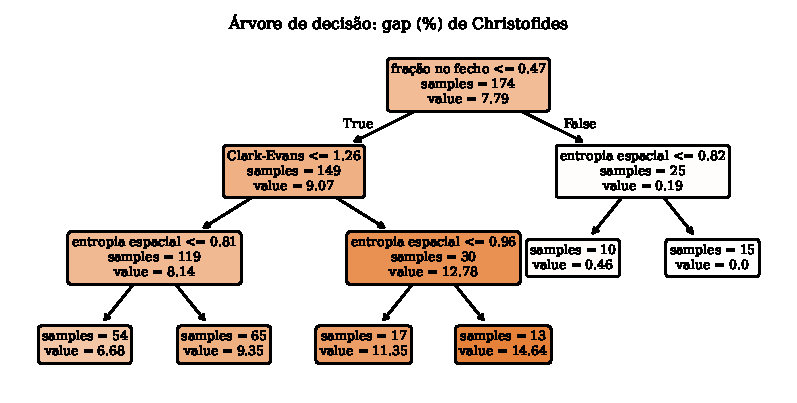
\includegraphics[width=\textwidth]{arvore_christofides}
\caption{Árvore de decisão (profundidade 3) para o gap do Christofides;
valor = gap médio (\%) da folha.}\label{fig:arvore}
\end{figure}

\paragraph{Por que a 1-árvore falhou no ulysses22.} O ulysses22 é o menor
$N$ em que o B\&B com 1-árvore estourou 30~minutos. Ele tem o maior CV da
distância ao vizinho mais próximo da TSPLIB (1,63; a mediana é 0,60) e um
dos maiores gaps de 1-árvore na raiz (30,6\%, igual ao do ulysses16 e
contra 9,6 a 19,7\% das instâncias com $N\ge24$). Os pontos são ilhas e
cidades do Mediterrâneo: grupos densos separados por grandes distâncias.
Nessa geometria, a MST junta cada grupo com arestas curtas e liga os grupos
com poucas arestas longas. Muitos vértices ficam com grau diferente de 2, e
a árvore está longe de um tour. O limite fica muito abaixo do ótimo em
todos os níveis, e quase nada é podado: foram de 44 a 57 milhões de nós
expandidos em 30~minutos, conforme a estratégia. O Held-Karp penaliza exatamente esses graus, deixou o gap na
raiz em 0,00\% e resolveu a instância com 20 nós.

\section{Conclusões}

\begin{itemize}
  \item \emph{Gargalos teóricos e práticos não coincidem.} O blossom segue
    a teoria ($N^{2{,}89}$, $R^2=0{,}997$) e domina o Christofides, de 81\%
    do tempo em $N=25$ a praticamente 100\% em $N=1000$. As rotinas
    $O(n^2)$ vetorizadas, por outro lado, crescem como $N^{1{,}2}$ até
    milhares de vértices, porque o custo por iteração do interpretador
    domina. Pelo mesmo motivo, o atalho das folhas, assintoticamente
    melhor, foi mais lento que o Prim em lote.
  \item \emph{Memória.} O que distorce a memória são cópias e estruturas
    de objetos: o grafo completo do NetworkX e a fila do best-first. O
    garbage collector não muda nenhum expoente (variação $\le0{,}02$) e
    quase não roda no B\&B em DFS. A troca de best-first por DFS levou a
    memória do B\&B de centenas de MiB para dezenas de KiB.
  \item \emph{Warm-start.} O efeito depende da ordem de visita dos filhos.
    Com filhos em ordem cega, a inserção a partir do fecho convexo reduziu
    a árvore em 41$\times$ e o tempo total de 5464~s para 102~s, a um custo
    de 0,5~ms. Com filhos ordenados pelo limite, a primeira descida já faz
    o papel da heurística, e o UB inicial quase não importa; com
    Held-Karp, um UB melhor chegou a gerar árvores \emph{maiores}. Em todos
    os casos, as heurísticas custam milissegundos e compensam sempre que a
    poda depende do UB.
  \item \emph{O limite inferior decide o ponto de colapso.} Com 1-árvore, o
    B\&B colapsa a partir de $N=22$ em instâncias agrupadas (ulysses22),
    nas quais o limite fica 30\% abaixo do ótimo. Com Held-Karp, o gap na
    raiz fica abaixo de 1\% e todas as instâncias até $N=70$ foram
    resolvidas.
  \item \emph{Features.} A fração de pontos no fecho convexo é a feature
    mais consistente: mais pontos no fecho significa gaps menores. A
    regularidade espacial (Clark-Evans e entropia) piora o Christofides, e
    a ramificação da MST (fração de vértices ímpares) piora o vizinho mais
    próximo e o TATT. As features globais explicam de 30 a 58\% da
    variância do gap em validação cruzada e 83\% do gap do limite de
    1-árvore. O restante depende de efeitos combinatórios locais.
\end{itemize}

Como trabalhos futuros, ficam três frentes: quebrar a simetria de reversão
do tour, o que reduziria a árvore pela metade; implementar o matching em
código compilado, que é o gargalo do Christofides; e usar características
de instância mais locais, que poderiam explicar a parte do gap que as
globais não explicam~\cite{smithmiles2012}.


\bibliographystyle{sbc}
\bibliography{referencias}


\end{document}
